\section{Introduction}

This lab attempts to verify the relation between various factors affecting centripetal motion and the centripetal force on a swinging mass.

\section{Procedure}

A support rod was attached to the side of a stable table.
The force sensor was affixed to the support rod, and the bob was dangled on the end of a string from the sensor.
A photogate was set up at the bottom of the construction, so that the bob would pass by the sensors as it swung.

\begin{figure}[h]

\begin{center}
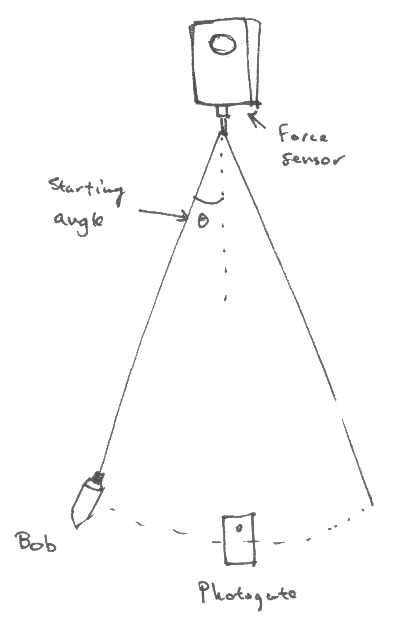
\includegraphics[scale=0.3]{content/fig1}
\end{center}

\caption{The setup of this lab.}

\end{figure}

For each of the tests, the distance from the sensor to the bob was recorded as the radius of the curve,
and the starting angle of the swing was recorded.

The distances and angled were adjusted throughout the experiment to get a range of readings.

\section{Results and Discussion}

\subsection{Questions}

\begin{enumerate}

\item Draw a free-body diagram of the pendulum. What is the direction of the net force on the pendulum?

\begin{figure}[h]

\begin{center}
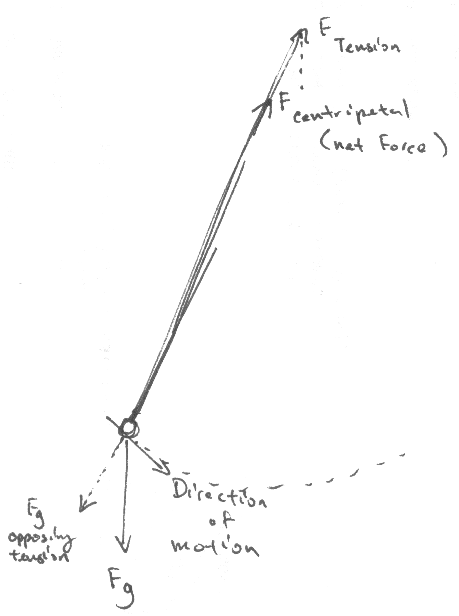
\includegraphics[scale=0.3]{content/fig2}
\end{center}

\caption{Free-body diagram for the system.}

\end{figure}

\item What is the acceleration of the pendulum as a function of time?

Beginning from the basic centripetal acceleration equation:

\begin{equation}a = \frac{v^2}{r}\end{equation}

We can use \begin{math}v = \frac{2 \pi r}{t}\end{math} to perform a substitution, and thus get:

\begin{equation}a = \frac{4 \pi^2 r}{t}\end{equation}

\item How does this acceleration correspond to the velocity of the pendulum?

From the first equation, we can see that the acceleration increases with the square of the velocity.

\item How does the acceleration vary with the length of the pendulum?

As the first equation implies, the acceleration decreases proportionally as the length of the pendulum increases.

\item What is the period of this circular motion (in seconds)?
How did you measure or calculate it?

Given that the angular velocity \begin{math}\omega = \frac{2\pi}{T}\end{math}, where T is the period of the revolution,
we can rearrange the equation such that:

\begin{equation}T = \frac{2\pi}{\omega}\end{equation}

Since we know the angle and how long it takes per swing, we can calculate \begin{math}\omega\end{math} by dividing the values.

\end{enumerate}

\subsection{Error Analysis}

The force sensor used was in itself a fairly large source of error in the measurements --- the measurements resulting from it were often fairly far off from the expected values, as calculated manually.

Additionally, measurements to the radius used may have been slightly off since it was difficult to measure to the exact same point on the bob each time.
This was probably a very small influence on the resulting calculations, though.

The last point of contention was in the size of the angles we used.
In theory, for most of the tests, the angle was quite small, and thus the influence of gravity on the system when the bob was not perfectly vertical should have been minimized.
Thus, the calculations generally assumed that the influence was negligible --- however, in truth, the larger the starting angle is, the larger the influence gravity would have on the experiment.

\section{Conclusion}

The experiment successfully showed, through the data, that increasing the velocity of the bob would necessitate a stronger centripetal force to keep the system rotating in a roughly circular fashion.

